\documentclass[12pt,letterpaper]{article}
\usepackage{fullpage}
\usepackage[top=2cm, bottom=4.5cm, left=2.5cm, right=2.5cm]{geometry}
\usepackage{amsmath,amsthm,amsfonts,amssymb,amscd}
\usepackage{lastpage}
\usepackage{enumerate}
\usepackage{fancyhdr}
\usepackage{mathrsfs}
\usepackage{xcolor}
\usepackage{graphicx}
\usepackage{listings}
\usepackage{hyperref}

\hypersetup{%
  colorlinks=true,
  linkcolor=blue,
  linkbordercolor={0 0 1}
}
 
\renewcommand\lstlistingname{Algorithm}
\renewcommand\lstlistlistingname{Algorithms}
\def\lstlistingautorefname{Alg.}

\lstdefinestyle{Python}{
    language     = Python,
    aboveskip    = 3mm,
    belowskip    = 3mm,
    frame        = lines, 
    basicstyle   = \footnotesize\ttfamily,
    keywordstyle = \color{blue},
    stringstyle  = \color{green},
    commentstyle = \color{red}\small\ttfamily
}

\setlength{\parindent}{0.0in}
\setlength{\parskip}{0.05in}

% Edit these as appropriate
\newcommand\course{CSE 3500}
\newcommand\hwnumber{3}                  % <-- homework number
\newcommand\NetIDa{mfm19005}           % <-- NetID of person #1

\pagestyle{fancyplain}
\headheight 35pt
\lhead{\NetIDa}
\chead{\textbf{\Large Homework \hwnumber}}
\rhead{\course \\ \today}
\lfoot{}
\cfoot{}
\rfoot{\small\thepage}
\headsep 1.5em

\newtheorem*{thm}{Theorem}

\begin{document}

\begin{center}
    \LARGE Problem Set
\end{center}


\section*{Problem 0 -- Dynamic Programming (25\%)}
Zoe starts at the top left corner of an $n \times n$ square grid of numbers and must end at the bottom right corner.
The numbers can be positive or negative. 
At each step, Zoe can go left, right, or down (but not up), and she can never revisit a square that she has already visited. 
Find an $O(n^2)$ algorithm to find the maximum sum of numbers Zoe can visit.\\

\par\noindent\rule{\textwidth}{0.4pt}

$\hfill \break$
An $O(n^2)$ algorithm that models this problem utilizes memoization in order to avoid repeated iterations. This algorithm uses a double for-loop in order to fill out an $n \times n$ table in which $T[i][j]$ represents the number of possible move directions that can be taken, given the conditions specified in the problem statement. Further, the algorithm iterates over all of the columns, except for the last one since the only possible move would be moving down for the last column.

$\hfill \break$
With this, we can iterate down each of the rows in order to compute the number of possible directions for each tile. This can be done by summing the number of possible directions for the tile to the right of the current one, and the tile below the current one. We can do this by going from the bottom up, and assembling the rows one by one. In this case, the bottom row must be all ones, since you can only go right in order to reach the goal - likewise, we can assemble upwards and use that bottom row in order to compute the row above it, and then set the ``below" row to the current row when moving up a level.

$\hfill \break$
Once the entire table is filled, we can iterate through and compute the maximum sum of numbers that Zoe can visit. This can be done by iterating through the table and summing the numbers in the table, and then comparing the sum to the current maximum sum. If the sum is greater than the current maximum sum, then we can set the maximum sum to the current sum.

$\hfill \break$
All of these operations will constitute the $O(n^2)$ we are looking for, as the initial construction of the table will cost $O(n^2)$ time, and the computation of the maximum sum will cost $O(n)$ time. Thus, the total time complexity will be $O(n^2)$.

\newpage

\section*{Problem 1 -- Divide and Conquer (25\%)}
A mad scientist accidentally left her cloning machine on and open while vacationing in Storrs, Connecticut.
While she was away, a murder of crows managed to get inside her office and use the cloning machine.
The mad scientist returned from her vacation surprised to have her office full of crows, but excited to test a new hypothesis.
As is well known, crows are very intelligent birds, and the scientist suspects that one or more crows may have taken advantage of the cloning machine to gain a selective genetic advantage.

We say that two crows are \textit{identical} if we genetically sequence the crows and their DNA is 99.99\% identical.
The mad scientist has a machine that will determine whether or not two crows are genetically identical, but it is costly to operate so she wants to minimize its use.

The only operation you are allowed to perform is to take two crows and determine if they are genetically identical.
Develop an $O(n \log n)$ algorithm that, given $n$ crows, determines if there is a set of more than $n/2$ crows that are genetically identical.

\par\noindent\rule{\textwidth}{0.4pt}

An $O(nlogn)$ equation that models this problem would be a derivation of merge sort, in that we can consider the set of all crows, $\mathbb{C}$, an array of sorts, and the crows being elements in that array. We can then split the array in half until we are left with arrays of two elements. This is one level above the normal terminating-point of a typical merge-sort algorithm. When we are left with two elements per list, we can compare all of the pairs on the final level of the recursive tree, and as such determine if there is a majority by checking for matching pairs.

$\hfill \break$
By executing this process recursively back up the tree, we are able to determine if the set of $\frac{n}{2}$ genetically identical crows exists for a given sample set. As such, the splitting-aspect of this algorithm constitutes the $O(logn)$ component of the final runtime, and the merging aspect of the algorithm constitutes the $O(n)$ component of the final runtime. Thus, the final runtime of this algorithm is $O(nlogn)$ as $n$ operations must run for each of the $log(n)$ levels.  

\newpage

\section*{Problem 2 -- SillySort (25\%)}

Prove that SillySort(L) terminates and correctly sorts its input list of numbers $L$.

    \lstset{caption={A sorting algorithm only used by silly people.}}
    \lstset{label={lst:alg1}}
     \begin{lstlisting}[style = Python]
def sillysort(L):
    while true:
        if L is sorted:
            return L
        else:
            compute an arbitrary index i such that L[i] > L[i+1]
            swap L[i] and L[i+1]
    \end{lstlisting}

\begin{thm}
    SillySort eventually terminates and correctly sorts its input list of numbers.
\end{thm}

\begin{proof}
    According to the definition of silly sort, it must execute the following steps during each iteration to get closer to fully sorting the input list:

    \begin{enumerate}
        \item Check if the list is sorted, if it is return the list.
        \item If the list is not sorted, then compute an arbitrary index $i$ such that $L[i] > L[i+1]$.
        \item Swap $L[i]$ and $L[i+1]$.
    \end{enumerate}

    With this, we can derive the base case of this problem, which is when the altered list is completely sorted. When this is the case, the algorithm will terminate. Now, we can explore how to get closer to the base case.

    $\hfill \break$
    During each iteration of the algorithm, we can assume that the list is not finished being sorted yet, and that it continues. With this in mind, the algorithm will arbitrarily select an index $i$ such that $L[i] > L[i+1]$, and that the two will be swapped in order to get closer to the final sorted list. This is very similar to how bubble sort operates, except instead of going sequentially and ensuring the items are sorted, this will compute the indices arbitrarily which adds additional complexity to the analysis of this algorithm.
    
    $\hfill \break$
    In this way, the best case is $O(n^2)$ for this algorithm when the list is already sorted, as it just needs to verify the list is sorted. The worst case is is $O(..)$ when the list is in reverse, and the average case is the list is in random order.

    $\hfill \break$
    We can prove that this algorithm correctly sorts a list by introducing an inductive proof, wherein the base step demonstrates the algorithm correctly sorts a list of size $n=3$, and the inductive step demonstrates that the algorithm correctly sorts a list of size $n+1$ given that it correctly sorts a list of size $n$.

    $\hfill \break$
    The base step can be modelled when the list is a known size, such as $n=4$. We can show this if we let $L = \left\{1, 2, 4, 3\right\}$, in which case the list can be sorted in one iteration. On the first iteration of the silly sort algorithm, it will detect indices 2, 3 are out of order, and swap them. This will result in the list being sorted, and so the algorithm will terminate successfully.

    $\hfill \break$
    The inductive step can be modelled when the list has an arbitrary size, $n+1$. We know that the algorithm will terminate when the list is sorted, and so we can assume that the list is not sorted. We can also assume that the algorithm will correctly sort a list of size $n-1$ given that it correctly sorts a list of size $n$. With this, we can assume that the algorithm will correctly sort a list of size $n$ given that it correctly sorts a list of size $n-1$. Therefore, the algorithm will process all pairs for which $L[i] > L[i+1]$, and swap them. This will result in the list being procedurally sorted, and so the algorithm will eventually terminate successfully.
\end{proof}

\newpage

\section*{Problem 3 -- Data structures (25\%)}

\begin{enumerate}
    \item We saw in class the algorithm for building a max-heap

    \lstset{caption={Building a max heap.}}
    \lstset{label={lst:alg1}}
     \begin{lstlisting}[style = Python]
import math

def buildmaxheap(A):
    A.heapsize = A.length
    for i in range(int(math.floor(A.length / 2)), 0, -1):
        maxheapify(A, i)
    \end{lstlisting}

Consider the following alternative way to build a max-heap

    \lstset{caption={Building a max heap.}}
    \lstset{label={lst:alg1}}
     \begin{lstlisting}[style = Python]
def buildmaxheap2(A):
    A.heapsize = 1
    for i in range(2, A.length + 1):
        maxheapinsert(A, A[i])
    \end{lstlisting}

    Prove that buildmaxheap and buildmaxheap2 do not always create the same heap by providing a counterexample.

    \begin{center}
        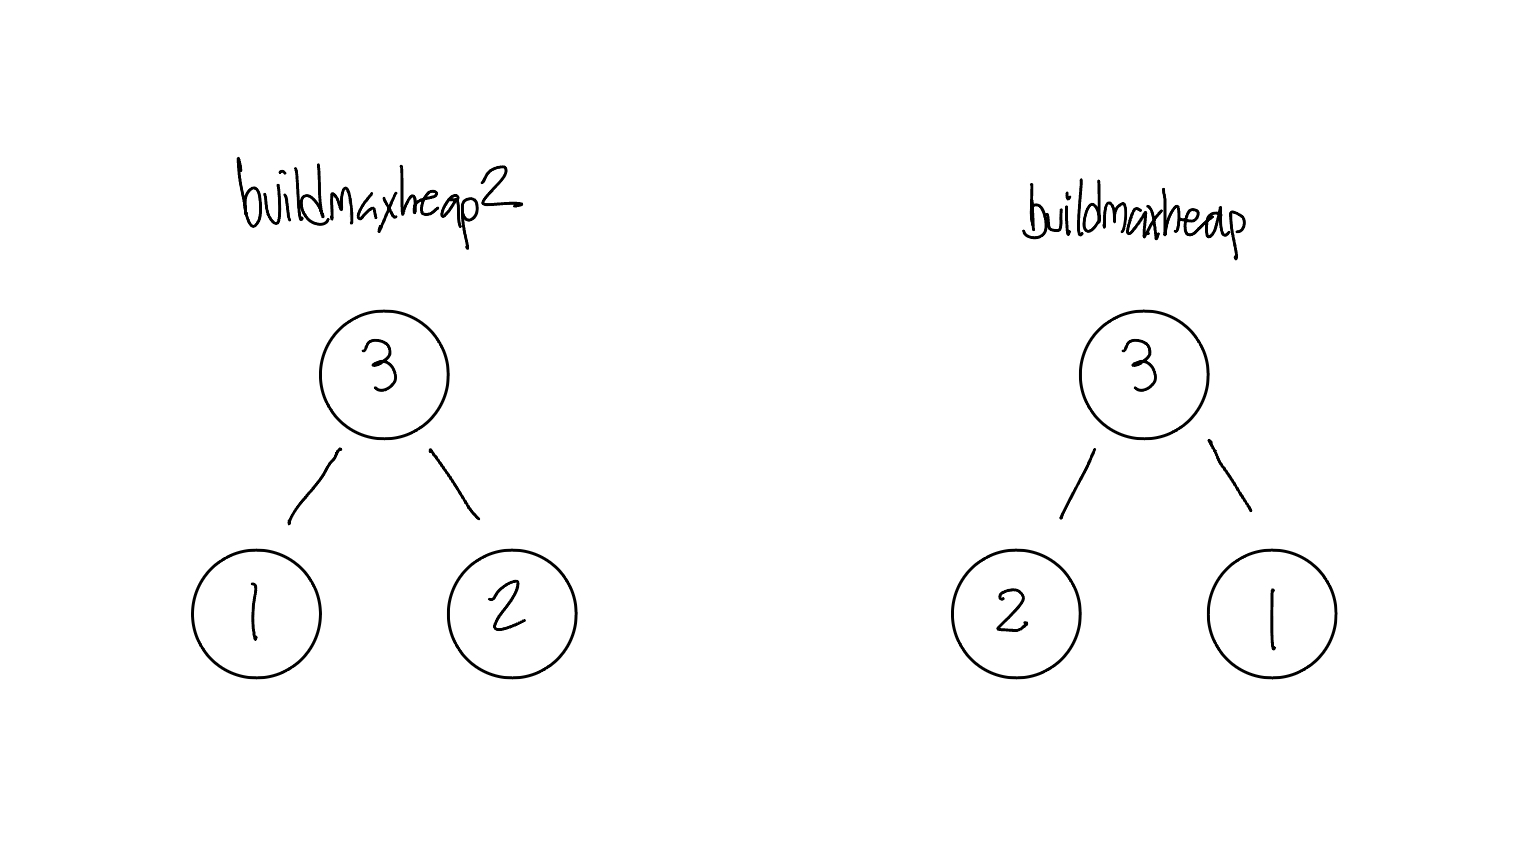
\includegraphics[height=7.5cm]{heaps.jpeg}
    \end{center}

    The above example, with \textit{buildmaxheap2} on the left, and \textit{buildmaxheap} on the right, demonstrates the case $\left[1, 2, 3\right]$ for each of the above functions. We can see that the generated results are visibly different with \textit{buildmaxheap2} generating $\left[3, 1, 2\right]$ and \textit{buildmaxheap} generating $\left[3, 2, 1\right]$.

    \item What is the worst case time complexity of buildmaxheap2? Explain your reasoning.
    \vspace{0.15cm}

    The worst case time complexity of \textit{buildmaxheap2} must be $O(nlogn)$. This is due to the fact that the function \textit{maxheapinsert} has a worst case time complexity of $O(logn)$, and the function is called $n$ times. Therefore, the worst case time complexity of \textit{buildmaxheap2} is $O(nlogn)$.
\end{enumerate}

\end{document}
